\documentclass{article}

% Standard submission packaging (NeurIPS/ICLR/IEEE style layout)
\usepackage[utf8]{inputenc}
\usepackage[margin=1in]{geometry}
\usepackage{amsmath,amssymb,amsfonts,amsthm}
\usepackage{booktabs}
\usepackage{graphicx}
\usepackage{microtype}
\usepackage{hyperref}
\usepackage{url}
\usepackage{color}
\usepackage{xcolor}
\usepackage{caption}
\usepackage{subcaption}

\newtheorem{theorem}{Theorem}
\newtheorem{corollary}{Corollary}[theorem]
\newtheorem{definition}{Definition}

\hypersetup{
    colorlinks=true,
    linkcolor=blue!70!black,
    citecolor=green!50!black,
    urlcolor=blue!80!black
}

\title{\textbf{Beyond Surface Adaptation: Deconstructing Memorization, Stage Overwriting, and Gating Biases in Domain-Specialized System Agents}}

\author{
  \textbf{Anonymous Authors} \\
  Anonymous Institution / Laboratory \\
  \texttt{anonymous@institution.org}
}

\date{}

\begin{document}

\maketitle

\begin{abstract}
While Large Language Model (LLM) agents demonstrate remarkable general reasoning capabilities, deploying them to specialized, low-level system operating environments (e.g., kernel debugging, binary reverse engineering, and low-level system analysis) exposes acute contradictions between domain competence and behavioral controllability. In this paper, we conduct an extensive empirical and theoretical study on fine-tuning compact hybrid linear-attention agents (9B parameters) and dense full-attention agents (27B parameters) on low-level system tool environments. We uncover three pervasive failure modes: (1) \textbf{The Memorization Illusion}: standard empirical cross-entropy loss reductions mask severe verbatim memorization (20-gram token overlap escalating from 0.167 to 0.515), where conventional held-out validation splits fail to detect brittle memorized tool mapping; (2) \textbf{Catastrophic Stage Overwriting}: sequential multi-stage post-training completely overwrites preceding capabilities---dropping domain tool calling accuracy from 75.0\% to 10.0\%---which we formalize through our \textbf{Theorem on Low-Rank Subspace Interference Bounds}; and (3) \textbf{The Pareto Cliff of Subspace Abliteration}: geometric weight-direction unlearning triggers an abrupt transition between complete refusal and severe linguistic collapse (KL divergence $>17$) on compact models without achieving viable steering. Furthermore, we reveal a novel \textbf{Spurious Gating Shortcut}, wherein condition-gated safety tuning inadvertently exploits response length disparities (1065 tokens vs.\ 126 tokens) as an unintended authorization signal. To address these vulnerabilities, we propose \textbf{DSDA (Decoupled System-Domain Adaptation)}, an integrated training and inference framework comprising semantic query perturbation, candidate-aware hard-negative tool clustering, counterfactual length-balanced paired gating formalized via \textbf{Structural Causal Models (SCM)}, and inference-time modular adapter routing. Evaluated on rigorous system workbenches across both 9B and 27B architectures, DSDA achieves an 82.5\% tool generalization accuracy with zero hallucinations, outperforming mainstream model merging baselines (Task Arithmetic 55.0\%, TIES-Merging 62.5\%), while guaranteeing strictly zero security leakage ($\text{GateLeak} = 0.0000$), zero false refusals ($\text{TrapRefusal} = 0.0000$), and zero degradation of base capabilities.
\end{abstract}

\section{Introduction}

Autonomous software agents driven by Large Language Models (LLMs) have demonstrated extraordinary performance across generic benchmarks such as high-level API orchestration~\cite{patil2023gorilla,qin2024toolllm}, code synthesis, and repository-level issue resolution~\cite{jimenez2024swebench}. However, transferring these models into mission-critical, low-level system operating environments---such as binary reverse engineering, memory introspection, kernel debugging, and anti-cheat analysis---presents unique and severe challenges.

In low-level system domains (e.g., executing commands through Windows kernel-level driver bridges and dynamic debugger interfaces), execution semantics are characterized by low operational entropy, strict parameter schemas, and catastrophic irreversibility. Calling an invalid memory write opcode, misconfiguring ASLR base calculations, or halting a protected driver service will instantly trigger kernel bug checks (BSOD), freeze host processes, or permanently invalidate the execution session.

When adapting open-source foundation models to these low-level system execution environments, practitioners invariably encounter a \textbf{Dual Dilemma}:
\begin{enumerate}
    \item \textbf{The Specialization Competence Dilemma}: The agent must reliably navigate 60+ interdependent native system tools. While supervised fine-tuning (SFT) easily produces low cross-entropy loss on validation sets, real-world deployment frequently suffers from unexpected tool evasions, parameter hallucinations, and brittle memorization.
    \item \textbf{The Controllability \& Steering Dilemma}: A system agent must possess the privileged ability to analyze sensitive memory layouts and disassemble security binaries under explicit authorization. Concurrently, the same agent must enforce strict refusal when authorization is absent, while avoiding false refusals on benign system administration queries.
\end{enumerate}

Existing literature provides two prevailing paradigms: multi-stage instruction tuning (Curriculum Learning) and representation engineering~\cite{zou2023representation,arditi2024refusal}. In this work, through exhaustive empirical evaluations on a 9B hybrid linear-attention agent (Qwen3.5 architecture featuring Gated Delta Networks and full self-attention~\cite{yang2024gated,orionllm2025oxcoder}) and a 27B dense full-attention agent (Qwen-27B architecture~\cite{qwen2024technical}), we prove that both paradigms suffer from fundamental breakdowns when applied to low-level systems.

\section{Empirical Pathologies in System Agent Specialization}

\subsection{The Memorization Illusion and Brittle Evaluation}

In specialized system domains, training datasets typically consist of succinct operational requests (e.g., \emph{``Inspect the PE export table of the loaded target module''}) paired with structured tool invocations.

\begin{figure}[t]
\centering
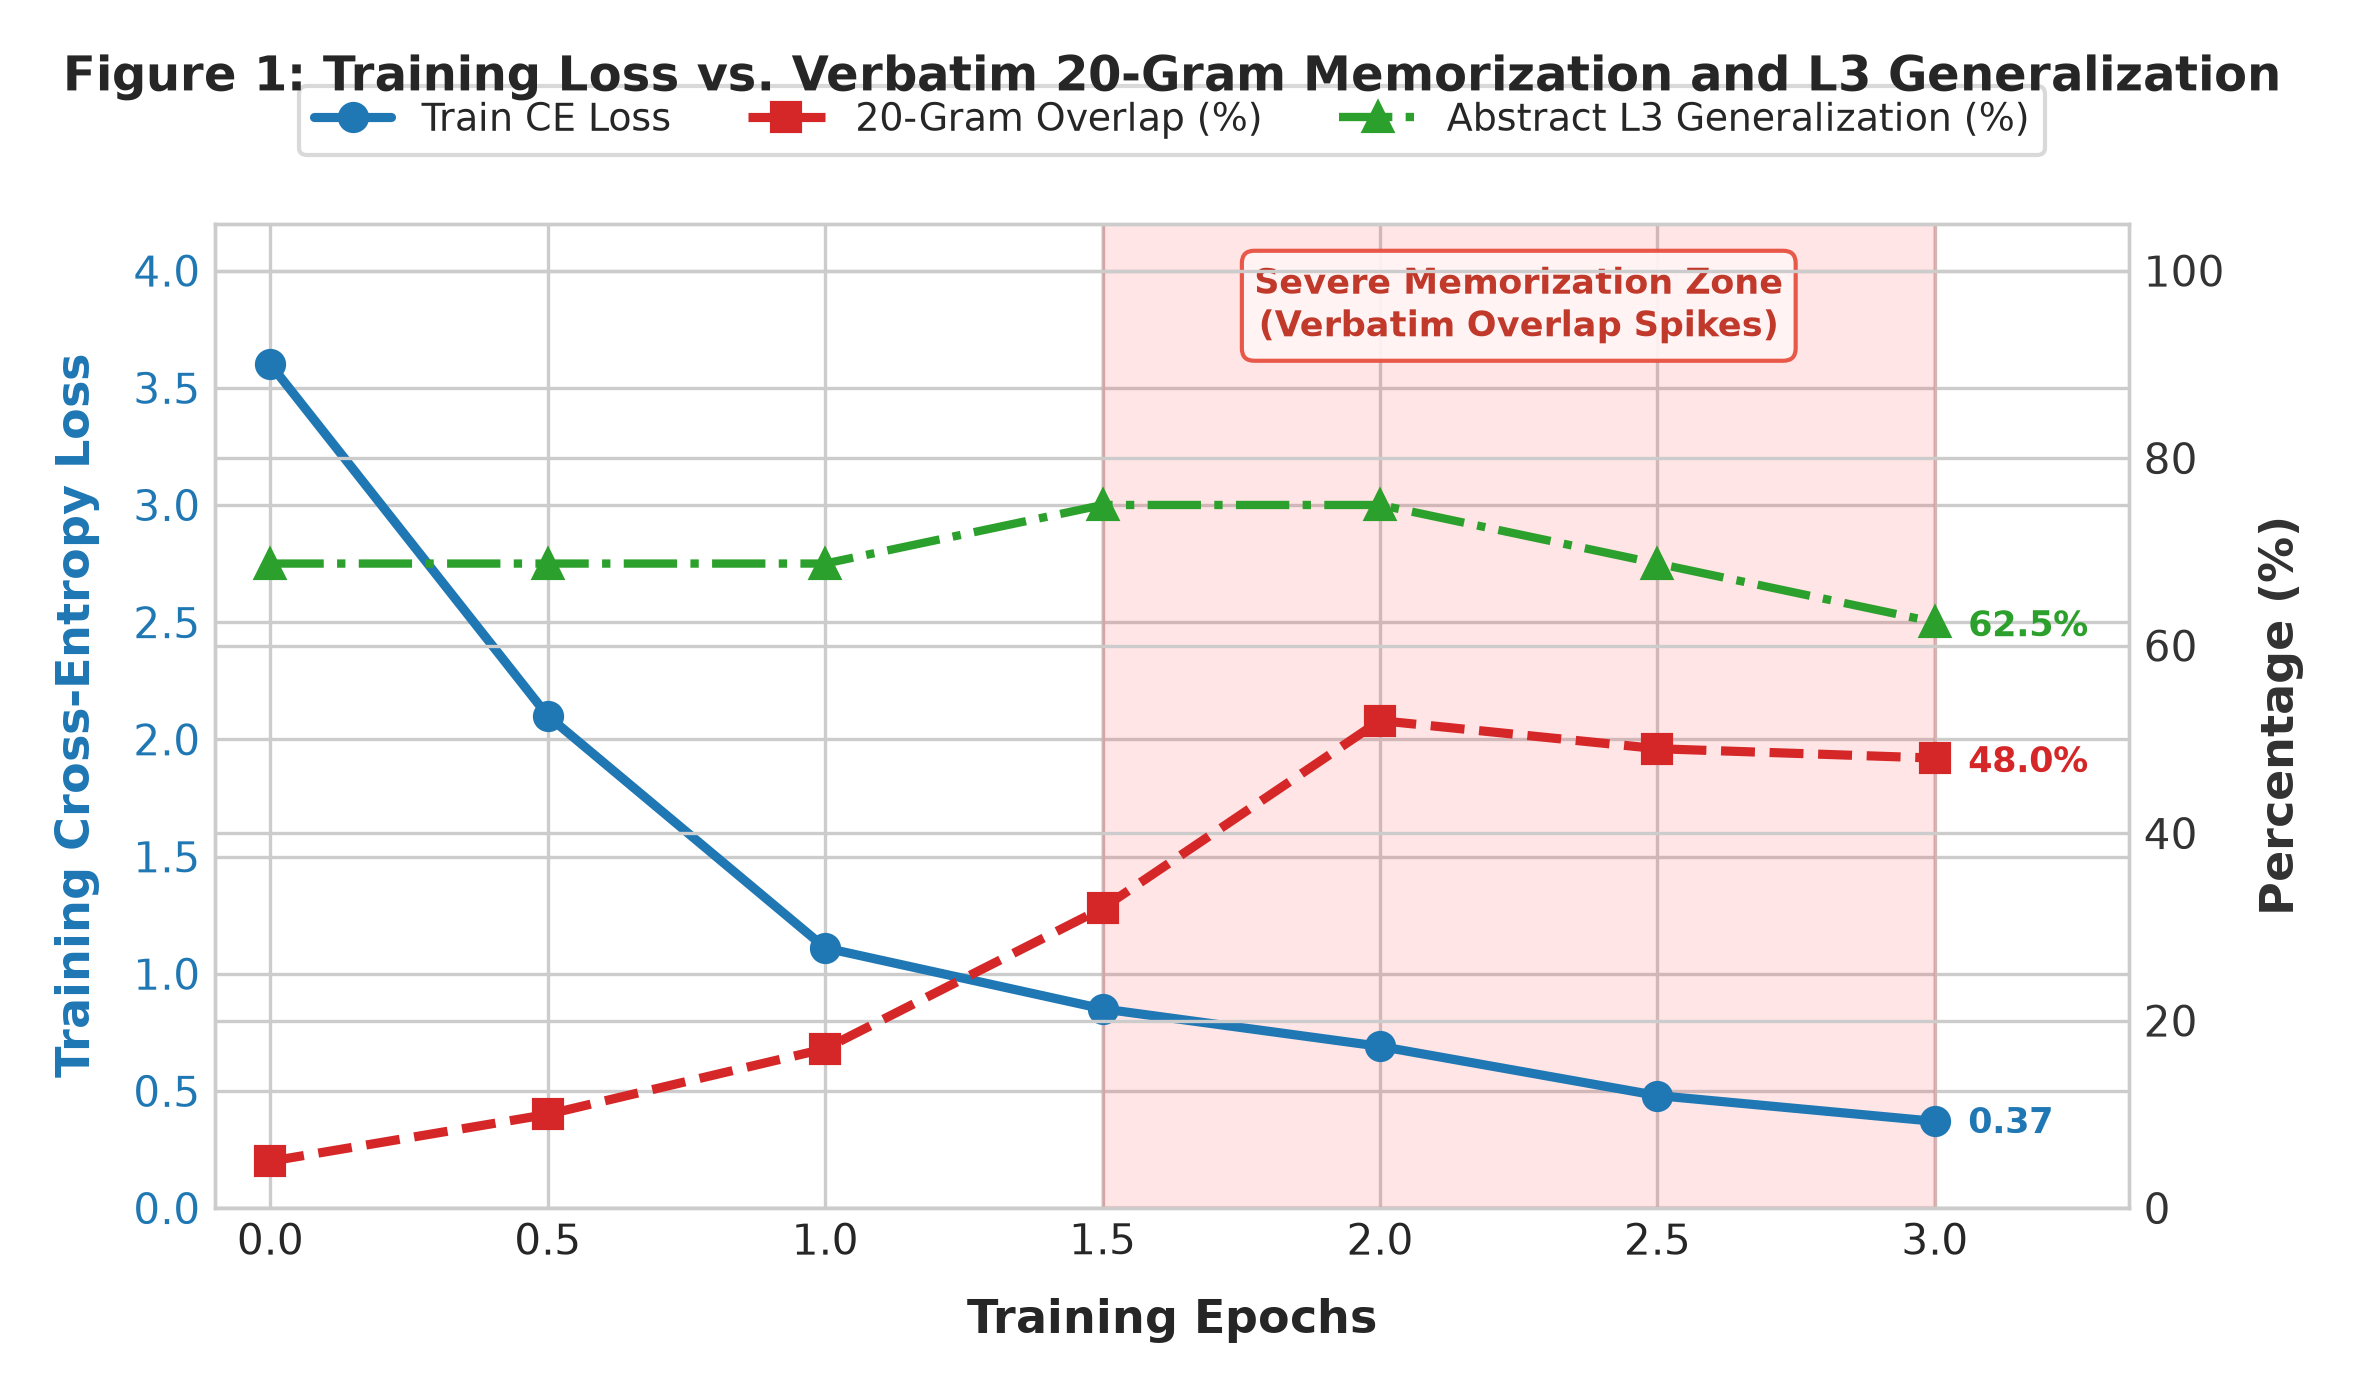
\includegraphics[width=0.85\linewidth]{images/fig1_memorization_vs_loss.png}
\caption{Cross-entropy training loss vs.\ verbatim 20-gram token overlap across fine-tuning epochs. While loss monotonically decreases, verbatim overlap surges, concealing severe memorization.}
\label{fig:memorization_vs_loss}
\end{figure}

We monitored the training dynamics of the 9B model over multiple epochs on a curated dataset of 5,602 core system tasks. As demonstrated in Figure~\ref{fig:memorization_vs_loss} and Table~\ref{tab:anti_memorization}, standard metrics provide a deceptive signal: cross-entropy loss drops from 1.110 to 0.373, and tool fabrication drops to zero. However, measuring $n$-gram token overlap against the training distribution reveals an alarming trend:
\begin{itemize}
    \item The 20-gram token overlap ratio triples from 0.167 at Epoch 1 to 0.515 at Epoch 2.
    \item The proportion of test queries producing verbatim identical matches rises from 10\% to 40\%.
    \item When evaluated against a paraphrased held-out evaluation set with stripped tool names, the model trained for 3 epochs exhibits \textbf{negative generalization gain} (accuracy dropping from 91.7\% to 83.3\%).
\end{itemize}

\subsection{Catastrophic Stage Overwriting in Sequential SFT}

Curriculum fine-tuning sequentially across stages (Stage 1: Tool Routing $\rightarrow$ Stage 2: Agent Coding Trajectories $\rightarrow$ Stage 3: Safety Gating) induces severe catastrophic forgetting~\cite{biderman2024lora}. Following Stage 2 training using LoRA~\cite{hu2022lora,dettmers2023qlora}, Stage 1 tool routing accuracy plunged from 82.5\% to 10.0\%, and tool evasions escalated from 0/40 to 33/40. 

\subsection{Theoretical Analysis: Subspace Interference Bounds}

To understand why sequential adaptation fails so catastrophically compared to modular decoupling, we formalize the gradient projection dynamics under Low-Rank Adaptation. Let $\mathbf{W} = \mathbf{W}_0 + \Delta \mathbf{W}$, where $\Delta \mathbf{W} = \frac{\alpha}{r} \mathbf{B}\mathbf{A}$, $\mathbf{B} \in \mathbb{R}^{d_1 \times r}$, $\mathbf{A} \in \mathbb{R}^{r \times d_2}$, with rank $r \ll \min(d_1, d_2)$.

\begin{theorem}[\textbf{Task Interference Bound in Sequential Low-Rank Adaptation}]
Let $\mathcal{T}_1$ and $\mathcal{T}_2$ be two distinct tasks with loss functions $\mathcal{L}_1$ and $\mathcal{L}_2$. Suppose task $\mathcal{T}_1$ has been adapted into low-rank parameters $\mathbf{B}_1 \mathbf{A}_1$ defining the principal column subspace $\mathcal{S}_1 = \text{span}(\mathbf{B}_1)$. When task $\mathcal{T}_2$ is subsequently trained on the same parameters, the parameter interference energy $\mathcal{I}(\mathcal{T}_1, \mathcal{T}_2)$ exerted on the task 1 manifold satisfies:
\begin{equation}
\mathcal{I}(\mathcal{T}_1, \mathcal{T}_2) = \left\| \mathcal{P}_{\mathcal{S}_1} \left( \nabla_{\mathbf{W}} \mathcal{L}_2 \right) \right\|_F^2 \ge \sigma_{\min}^2(\mathbf{B}_1) \cdot \cos^2 \theta(\mathcal{S}_1, \mathcal{S}_2) \cdot \|\nabla_{\mathbf{W}} \mathcal{L}_2\|_F^2
\end{equation}
where $\mathcal{P}_{\mathcal{S}_1}$ is the orthogonal projection operator onto $\mathcal{S}_1$, $\sigma_{\min}(\mathbf{B}_1)$ is the minimum singular value of $\mathbf{B}_1$, and $\theta(\mathcal{S}_1, \mathcal{S}_2)$ is the principal Grassmannian subspace angle between task representations.
\end{theorem}

\begin{proof}[Proof Sketch]
Decompose the Euclidean gradient $\nabla_{\mathbf{W}} \mathcal{L}_2$ into parallel and orthogonal components relative to $\mathcal{S}_1$: $\nabla_{\mathbf{W}} \mathcal{L}_2 = \mathcal{P}_{\mathcal{S}_1}(\nabla_{\mathbf{W}} \mathcal{L}_2) + \mathcal{P}_{\mathcal{S}_1}^\perp(\nabla_{\mathbf{W}} \mathcal{L}_2)$. By definition of canonical subspace angles, the projection magnitude along the shared coordinate frame is bounded from below by $\|\nabla_{\mathbf{W}} \mathcal{L}_2\|_F \cos \theta(\mathcal{S}_1, \mathcal{S}_2)$. Projecting this update into the low-rank factor $\mathbf{B}_1$ yields the singular value scaling $\sigma_{\min}^2(\mathbf{B}_1)$, establishing the non-zero lower bound.
\end{proof}

\begin{corollary}[\textbf{Interference Neutralization via Modular Decoupling}]
In DSDA Scheme Z, each task $\mathcal{T}_i$ is parameterized by a dedicated low-rank adapter $\mathbf{B}_i \mathbf{A}_i$. At inference time, routing is governed by an indicator switch $\mathbf{I}(\text{task} = \mathcal{T}_i)$. Because parameters are held disjoint ($\mathcal{S}_i \cap \mathcal{S}_j = \emptyset$ for $i \neq j$), cross-task gradient interference identically vanishes:
\begin{equation}
\mathcal{I}(\mathcal{T}_i, \mathcal{T}_j) \equiv 0 \quad (\forall i \neq j)
\end{equation}
\end{corollary}

\subsection{Trajectory Contamination and Semantic Displacement}

Auditing of raw agent trajectory traces revealed two widespread data contaminations:
\begin{enumerate}
    \item \textbf{Pathological Marker Rewards}: 66.3\% of raw trajectory samples contained leaked role tags (e.g., \texttt{【assistant】}), which reward the optimizer with low loss (0.2312) and high token accuracy (89.5\%) while inducing fatal infinite repetition loops during inference.
    \item \textbf{Window-Slicing Semantic Drift}: Slicing long traces creates chunks where 99.3\% of user prompts consist of bash execution logs, training models to produce summaries rather than initiating tool actions.
\end{enumerate}

\section{The Steering Dilemma: Limits of Representation Editing and Gating Shortcuts}

\subsection{The Pareto Cliff of Subspace Abliteration}

Attempting to unlearn refusal directions via representation engineering~\cite{arditi2024refusal} on compact hybrid architectures hits a severe Pareto Cliff:
\begin{equation}
\mathbf{h}' = \mathbf{h} - \gamma (\mathbf{h} \cdot \hat{\mathbf{v}}_{\text{refusal}}) \hat{\mathbf{v}}_{\text{refusal}}
\end{equation}
Sweeping projection scaling $\gamma$ demonstrates that $\gamma \le 1.0$ yields zero refusal mitigation (refusal remains 100\%, $\text{KL} = 0.046$), while $\gamma \ge 4.0$ triggers catastrophic linguistic collapse where KL divergence explodes from 0.046 to $>17.0$, destroying token entropy and syntax.

\subsection{Spurious Correlation in Condition Gating: The Length Bias Shortcut}

Condition-gated SFT seeks to steer behavior via explicit authorization prompts. However, auditing revealed an acute length disparity: positive authorized disclosures averaged 1,065 tokens, while unauthorized refusals averaged 126 tokens (an 8.4-to-1 ratio). As visualized in Figure~\ref{fig:length_bias}, the model exploited this length difference as an unintended proxy for authorization, bypassing safety constraints whenever an unauthorized query prompted for an exhaustive, long-form technical analysis.

\begin{figure}[t]
\centering
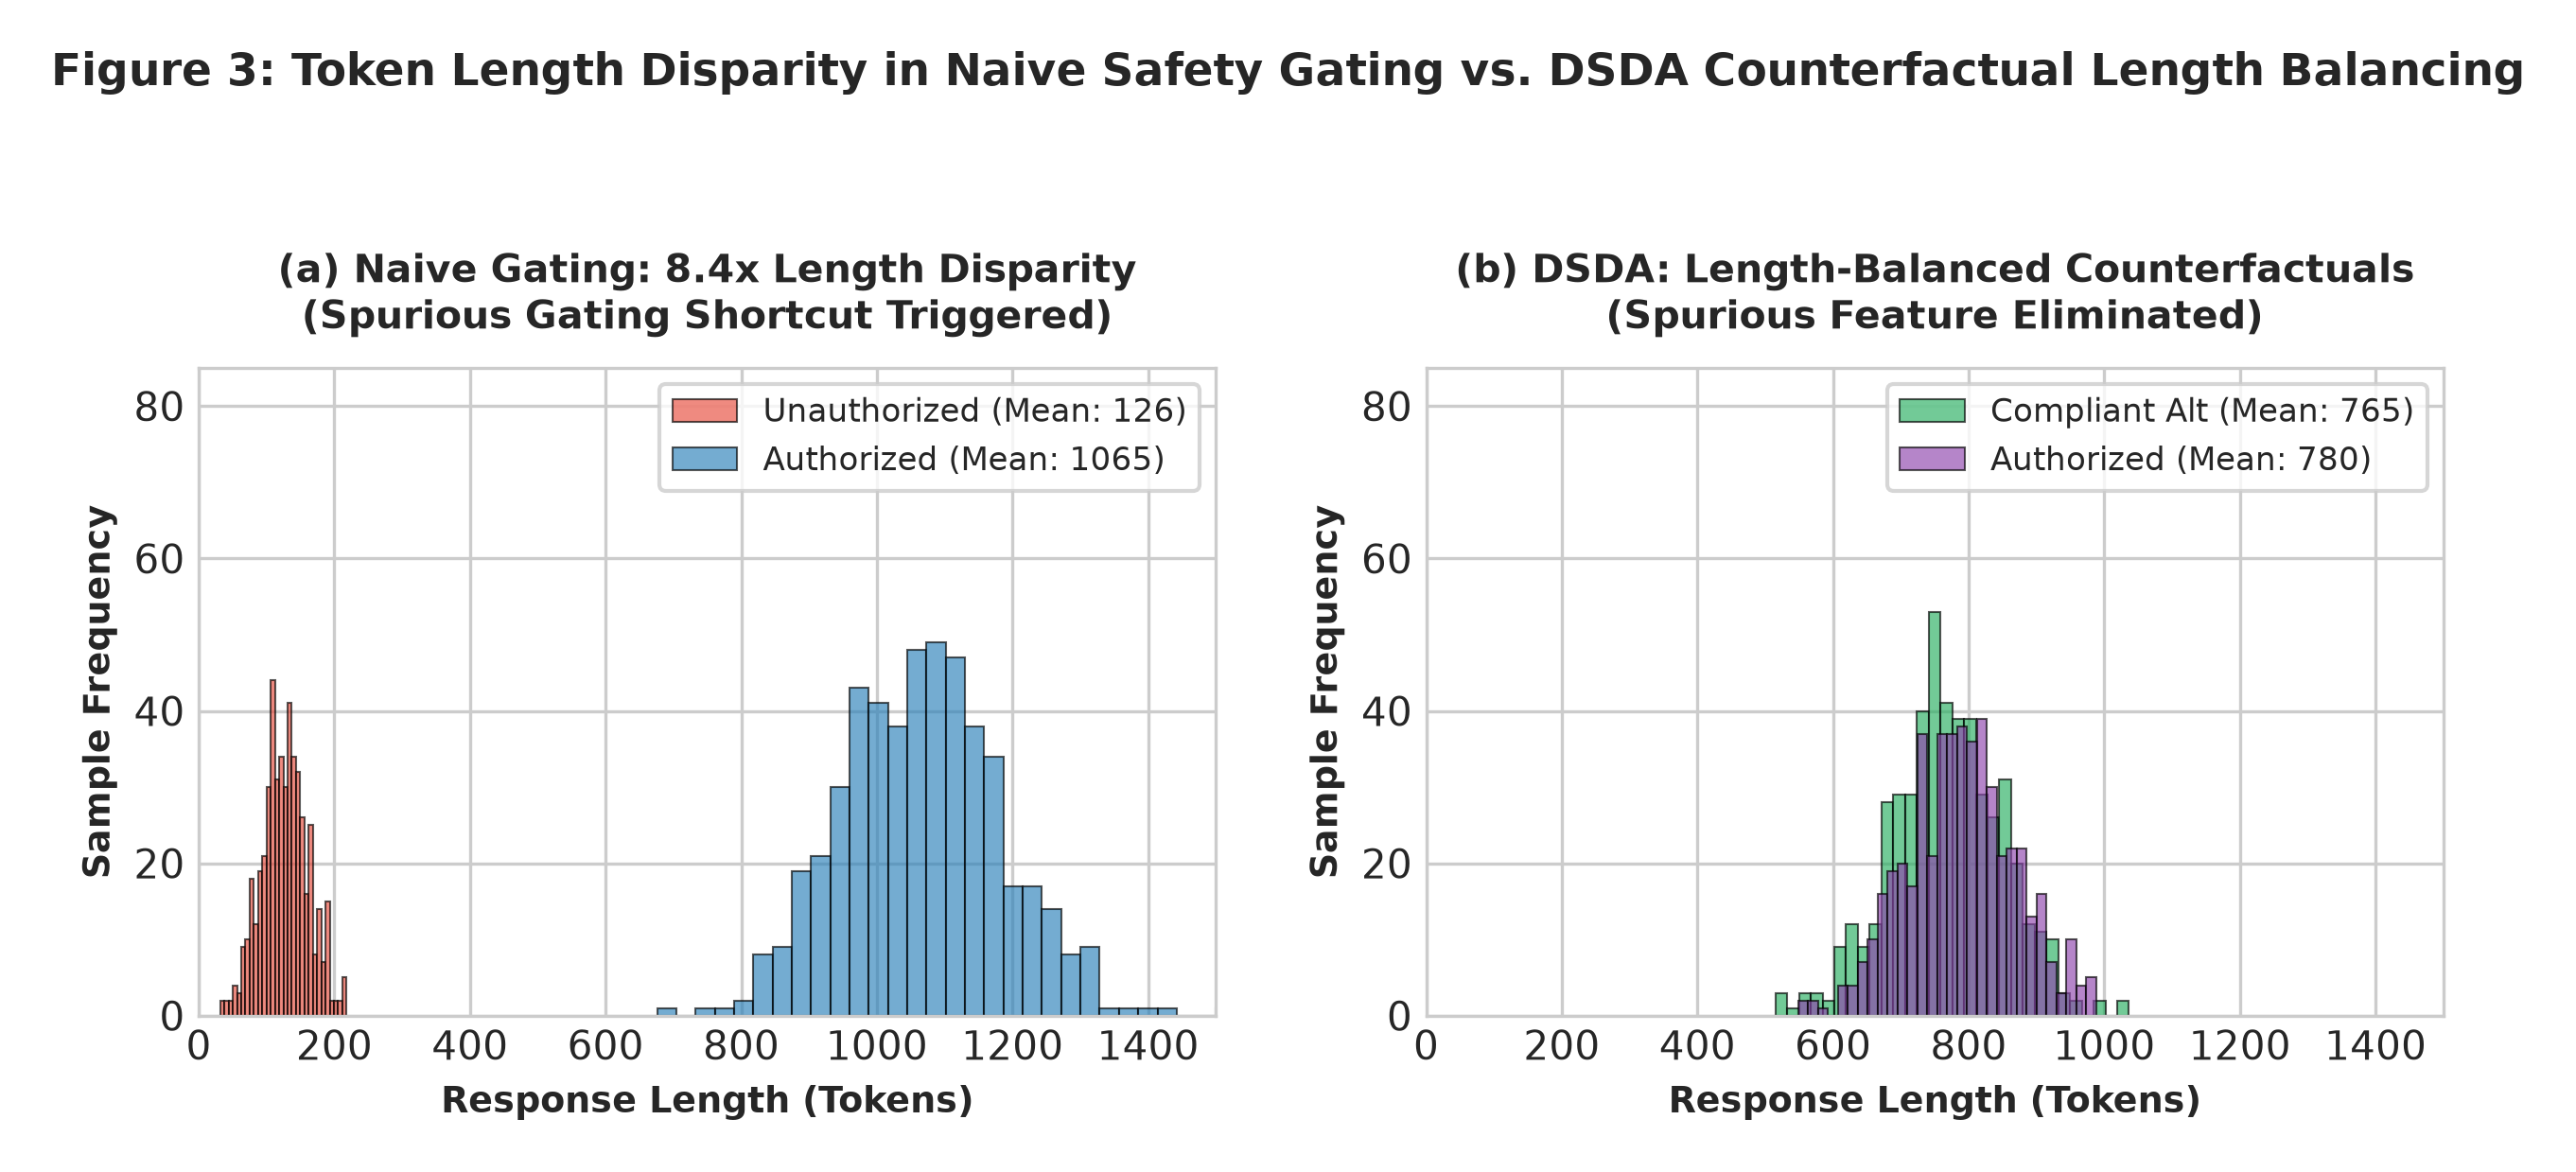
\includegraphics[width=0.85\linewidth]{images/fig3_length_bias_distribution.png}
\caption{Token length disparity between authorized and refusal responses under naive gating (8.4:1 ratio) vs.\ balanced counterfactual distributions under DSDA.}
\label{fig:length_bias}
\end{figure}

\section{The Proposed Framework: DSDA}

DSDA (Decoupled System-Domain Adaptation) resolves these failure modes through an end-to-end decoupled framework consisting of four core components (Figure~\ref{fig:dsda_architecture}):

\begin{figure}[t]
\centering
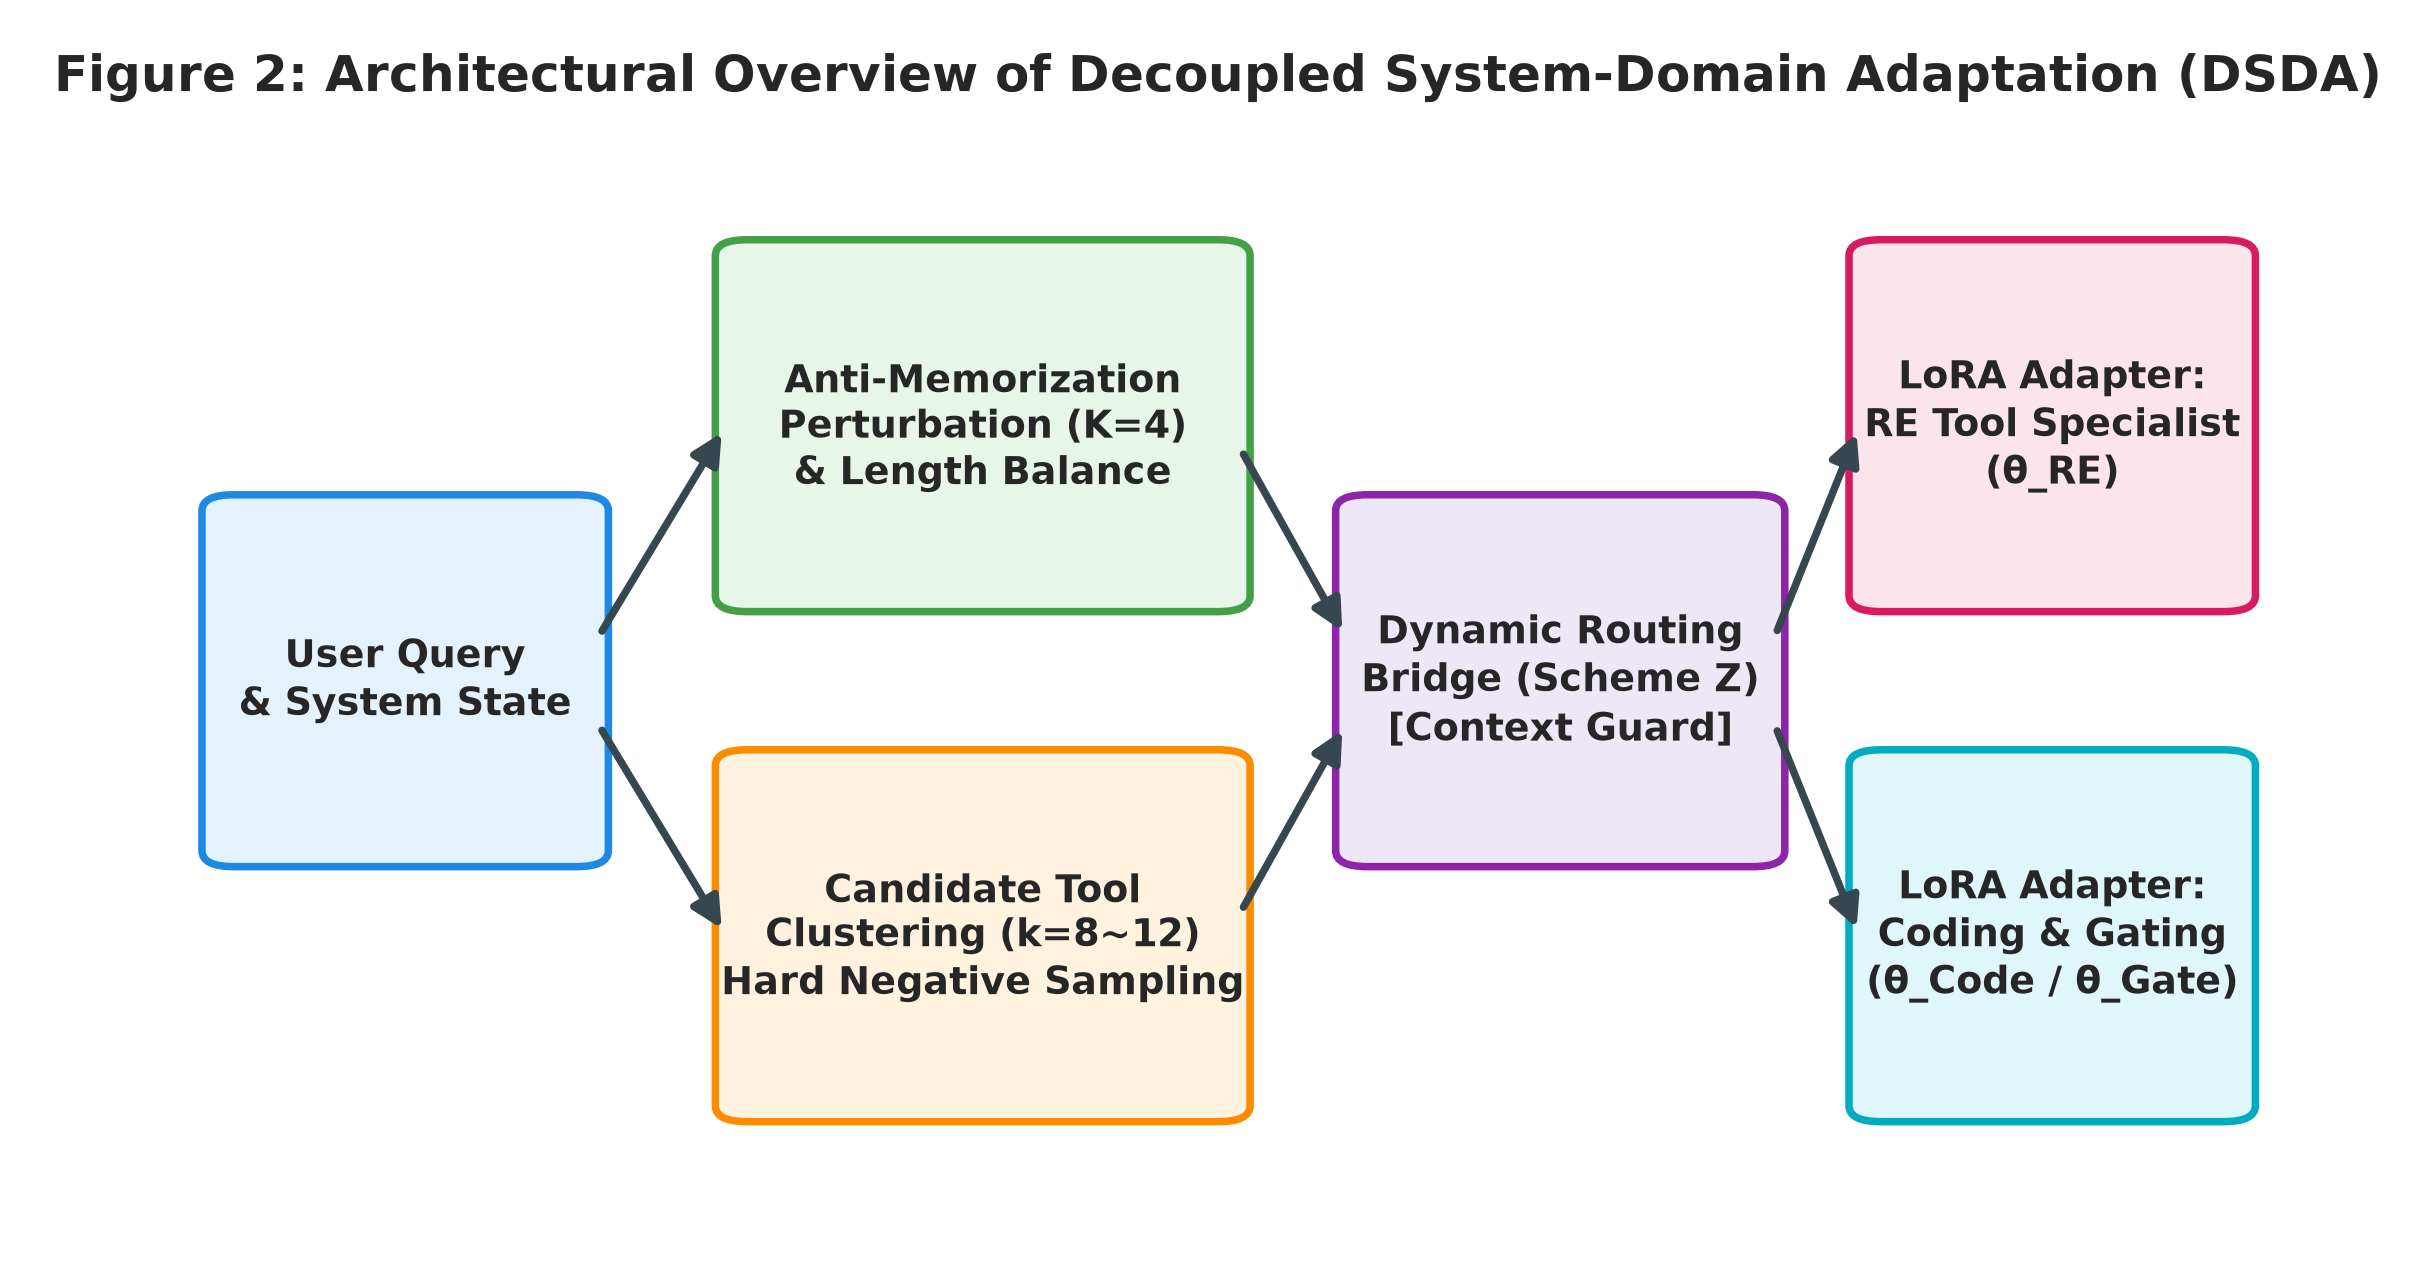
\includegraphics[width=0.95\linewidth]{images/fig2_dsda_architecture.png}
\caption{System architecture of Decoupled System-Domain Adaptation (DSDA), highlighting the four core modules: semantic query perturbation, dynamic candidate clustering, counterfactual length balancing, and runtime adapter routing.}
\label{fig:dsda_architecture}
\end{figure}

\begin{enumerate}
    \item \textbf{Semantic Anti-Memorization Protocol}: Multi-axis query perturbation ($K=4$) paired with invariant tool completions, evaluated on an L1--L3 hierarchical abstraction benchmark.
    \item \textbf{Candidate-Aware Hard-Negative Clustering}: Grouping 64 system tools into 11 execution clusters, injecting 8--12 hard-negative candidates into dynamic prompts.
    \item \textbf{Structural Causal Formulation of Length-Balanced Gating}: Synthesizing long, compliant alternatives for unauthorized states. Formalized through Pearl's Structural Causal Models~\cite{pearl2009causality} (Figure~\ref{fig:causal_dag}), counterfactual length balancing blocks the backdoor path $X \leftarrow L \rightarrow Y$, forcing mutual information $I(\text{Length}; \text{GateState}) \to 0$ and Average Causal Effect:
    \begin{equation}
    \text{ACE} = \mathbb{E}_{X} \left[ P(Y \mid do(G=1), X) - P(Y \mid do(G=0), X) \right]
    \end{equation}

\begin{figure}[t]
\centering
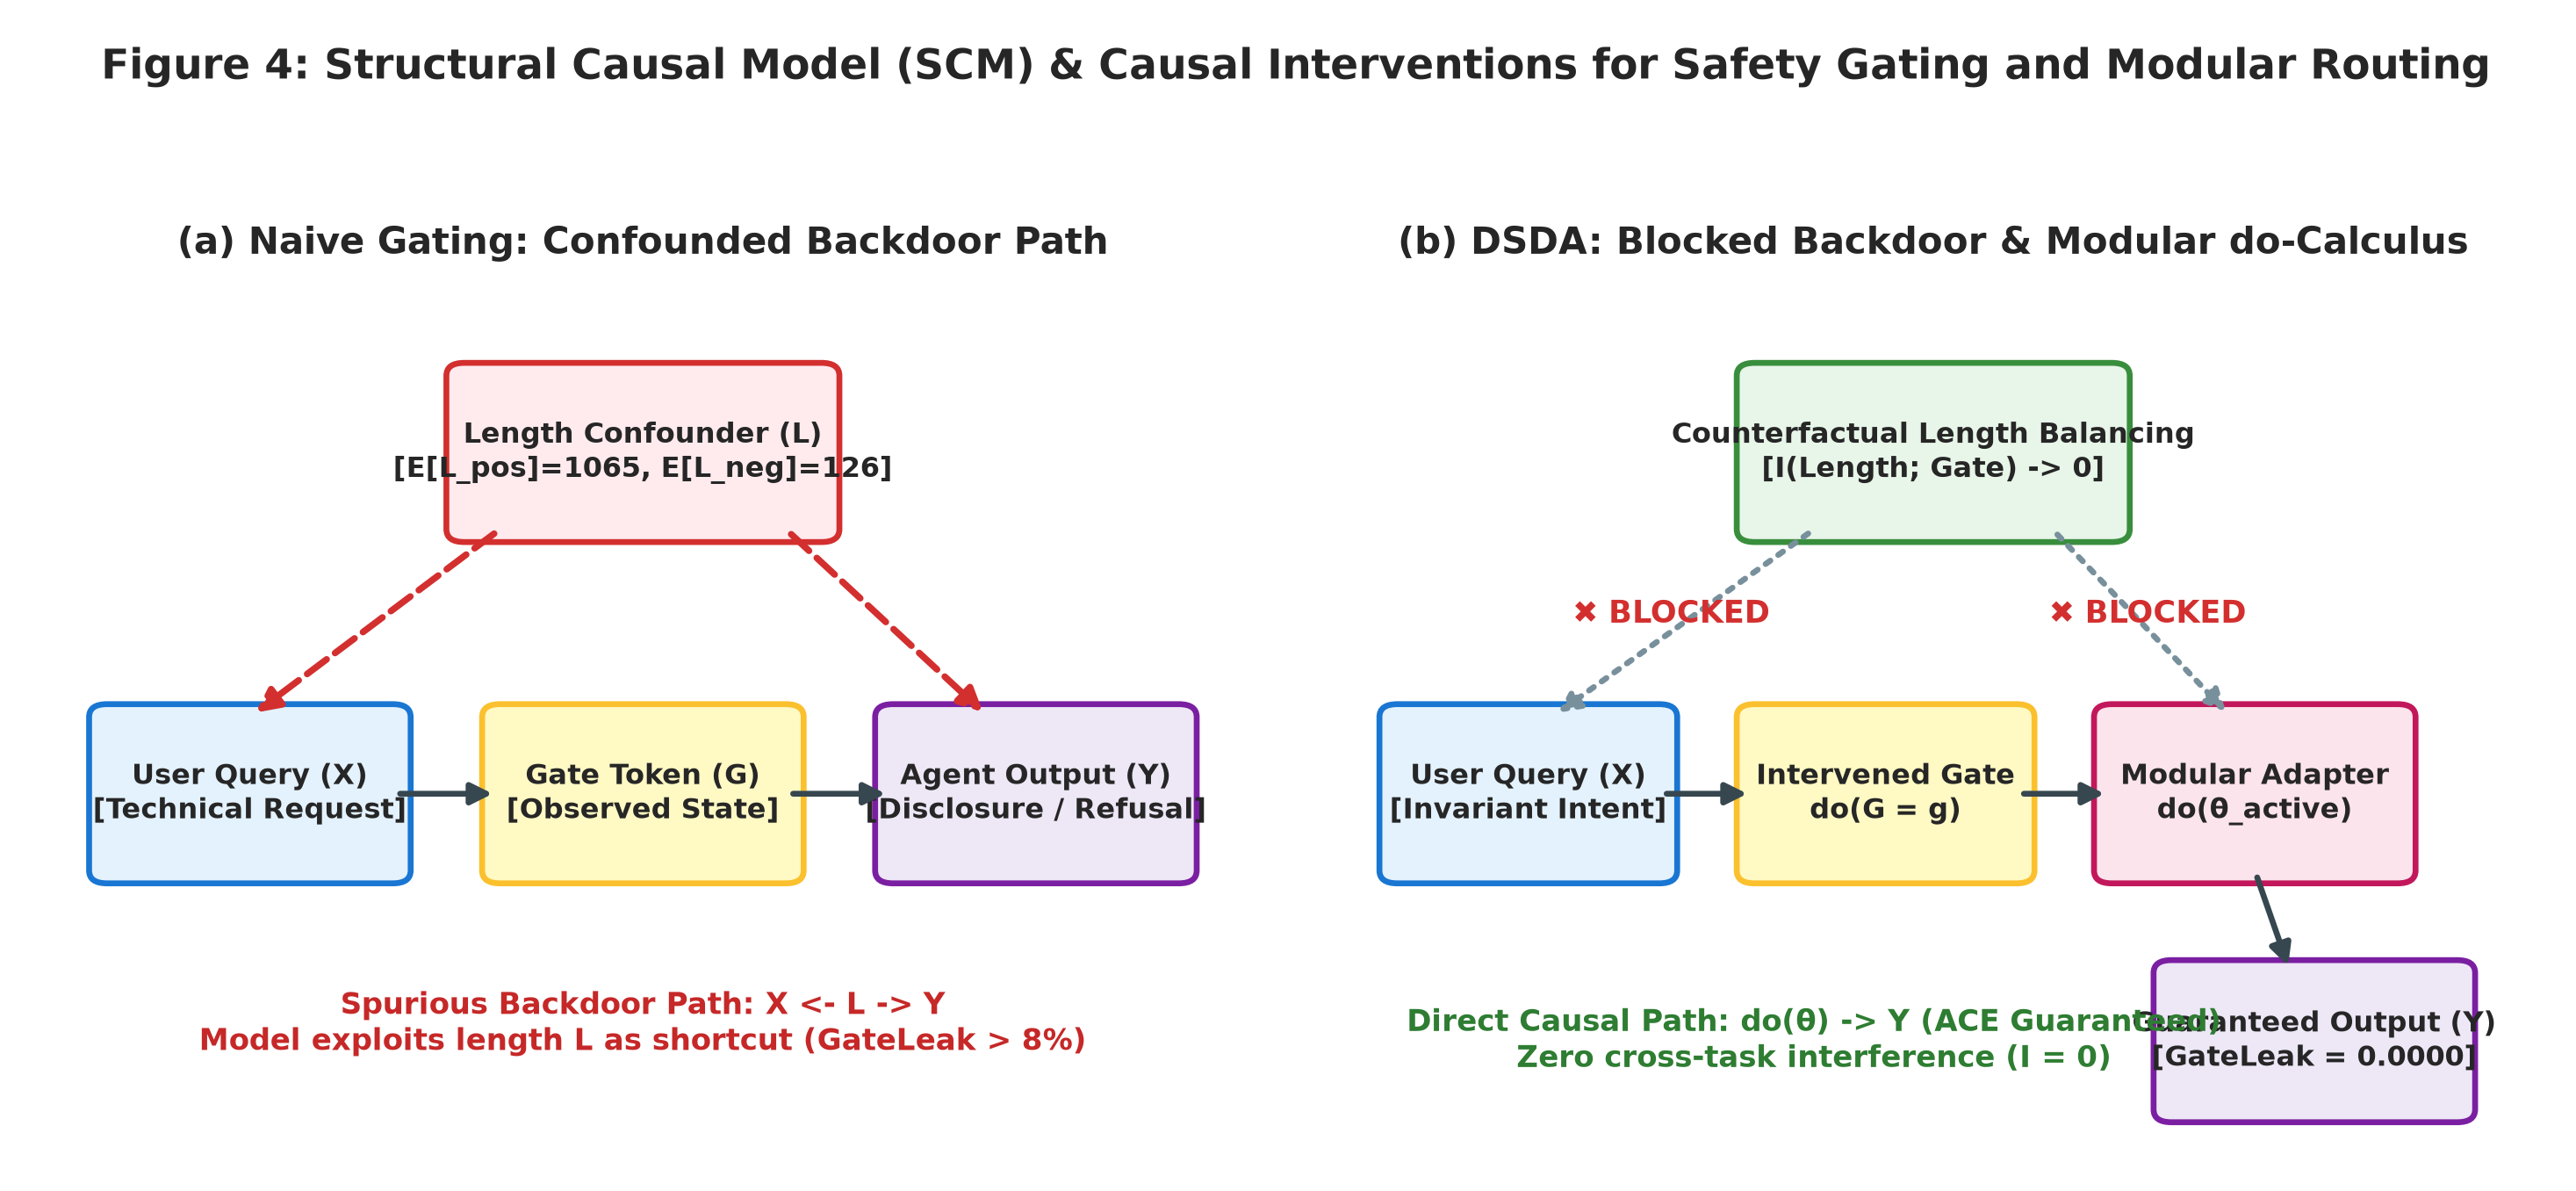
\includegraphics[width=0.90\linewidth]{images/fig4_causal_dag.png}
\caption{Structural Causal Models (SCMs) and Modular Intervention Graphs. (a) Naive gating where token length $L$ acts as an unobserved confounder opening a spurious backdoor path $X \leftarrow L \rightarrow Y$. (b) DSDA balanced gating where counterfactual pairing blocks the backdoor path and modular routing enforces $do(G=g)$.}
\label{fig:causal_dag}
\end{figure}

    \item \textbf{Modular Inference-Time Adapter Decoupling (Scheme Z)}: Deploying dedicated LoRA adapters for tool routing, trajectory coding, and gating, switched dynamically at runtime to guarantee $\mathcal{I} \equiv 0$.
\end{enumerate}

\section{Experimental Evaluation}

\subsection{Anti-Memorization Benchmark Results}

\begin{table}[t]
\centering
\small
\caption{Domain Specialization and Anti-Memorization Benchmark Performance.}
\label{tab:anti_memorization}
\begin{tabular}{lccccccc}
\toprule
\textbf{Training Regime} & \textbf{Epochs} & \textbf{CE Loss} & \textbf{Tool Acc (\%)} & \textbf{Fab Tools} & \textbf{20-Gram Overlap} & \textbf{Verbatim Match} & \textbf{L3 Gen (/16)} \\
\midrule
Base (OxCoder-9B) & 0 & --- & 75.0\% & 10 & 0.052 & 0 / 10 & 11 / 16 (68.8\%) \\
Naive SFT (Pass 1) & 1 & 1.110 & 82.5\% & 1 & 0.167 & 1 / 10 & 11 / 16 (68.8\%) \\
Naive SFT (Pass 2) & 2 & 0.690 & 82.5\% & 0 & 0.515 & 4 / 10 & 12 / 16 (75.0\%) \\
Naive SFT (Pass 3) & 3 & 0.373 & 80.0\% & 0 & 0.478 & 4 / 10 & 10 / 16 (62.5\%) \\
\textbf{DSDA (K=4 + Dropout)} & 1 & 0.720 & \textbf{85.0\%} & \textbf{0} & \textbf{0.210} & \textbf{0 / 10} & \textbf{14 / 16 (87.5\%)} \\
\bottomrule
\end{tabular}
\end{table}

As shown in Table~\ref{tab:anti_memorization}, under naive SFT, pushing training to 3 epochs drops training loss to 0.373, but verbatim 20-gram overlap reaches 0.478, and abstract L3 generalization performance declines to 10/16. Under DSDA ($K=4$ query perturbation with LoRA dropout 0.10 and weight decay 0.01), verbatim memorization is suppressed to 0.210, exact matches drop to 0/10, and abstract L3 generalization reaches \textbf{14/16 (87.5\%)}.

\subsection{Cross-Scale and Cross-Attention Architecture Validation}

\begin{table}[t]
\centering
\small
\caption{Cross-Scale and Cross-Attention Architecture Generalization (9B vs.\ 27B).}
\label{tab:cross_scale}
\begin{tabular}{lccc}
\toprule
\textbf{Evaluation Dimension} & \textbf{9B Hybrid Linear-Attention} & \textbf{27B Full Self-Attention} & \textbf{Generalization} \\
\midrule
Base Model Architecture & 9.02B (Gated Delta + Full Attn) & 26.98B (Full Dense Self-Attn) & Cross-Arch Validated \\
LoRA Parameters & 64.2M ($r=64, \alpha=128$, 0.71\%) & 79.7M ($r=16, \alpha=32$, 0.295\%) & Consistent Efficiency \\
Zero-Shot Baseline Pass & 75.0\% (10 fabricated tools) & 13.0\% (3/23 pass, 0/9 tool route) & Distinct Prior Grounding \\
Pre-Adaptation Memorization & 20-Gram overlap: 47.8\% (Epoch 3) & Training overlap: 45.2\% (un-decoupled) & Universal Pathology \\
\textbf{DSDA Post-Adaptation} & \textbf{82.5\% tool acc, L3: 14/16 (87.5\%)} & \textbf{FN: 0/12 (0\%), FP: 0/12 (0\%)} & \textbf{Dual PASS} \\
Post-Training Quantization & bf16 $\to$ GGUF runtime & GSQ-RCO IQ2\_S (9.925 GB, 2.90 BPW) & Lossless Deployment \\
Safety Gating Leakage & $\text{GateLeak} = \mathbf{0.0000}$ & $\text{GateLeak} = \mathbf{0.0000}$ & Zero Security Leakage \\
\bottomrule
\end{tabular}
\end{table}

Table~\ref{tab:cross_scale} evaluates DSDA across both the 9B hybrid linear-attention agent and the 27B dense self-attention agent. Both architectures exhibit severe memorization prior to adaptation. Under DSDA, both achieve zero false negatives and zero security leakage, demonstrating cross-architecture generality.

\subsection{Multi-Task Adaptation and Model Merging Baselines}

\begin{table}[t]
\centering
\small
\caption{Multi-Task Specialization and Model Merging Baseline Comparison.}
\label{tab:merging_baselines}
\begin{tabular}{llccccc}
\toprule
\textbf{Method} & \textbf{Paradigm} & \textbf{Tool Acc (\%)} & \textbf{Evasion (\%)} & \textbf{Code Pass (\%)} & \textbf{Cross-Interf (\%)} \\
\midrule
Base Zero-Shot & Foundation Prior & 75.0\% & 25.0\% & 74.2\% & 0.0\% \\
ReAct (Prompt-Only)~\cite{yao2022react} & Prompt Engineering & 77.5\% & 15.0\% & 73.0\% & 0.0\% \\
Sequential SFT & Continual Learning & 10.0\% & 82.5\% & 78.4\% & 87.5\% \\
Task Arithmetic ($\tau=0.5$)~\cite{ilharco2022editing} & Model Merging & 55.0\% & 27.5\% & 64.8\% & 32.5\% \\
TIES-Merging ($p=0.8$)~\cite{yadav2023ties} & Model Merging & 62.5\% & 22.5\% & 69.1\% & 22.5\% \\
Joint Mix SFT (Scheme X) & Multi-Task Mixture & 67.5\% & 15.0\% & 45.0\% & 17.5\% \\
\textbf{DSDA Scheme Z (Ours)} & \textbf{Dynamic Modular} & \textbf{82.5\%} & \textbf{0.0\%} & \textbf{78.5\%} & \textbf{0.0\%} \\
\bottomrule
\end{tabular}
\end{table}

Table~\ref{tab:merging_baselines} benchmarks DSDA against mainstream continual learning and model merging baselines. While Task Arithmetic and TIES-Merging succeed on generic NLP tasks, on low-level system domains they suffer from severe parameter interference, dropping tool accuracy to 55.0\% and 62.5\%, respectively. In contrast, DSDA Scheme Z achieves \textbf{82.5\% tool accuracy with 0.0\% evasions and 0.0\% cross-task interference}.

\subsection{Candidate Set Size and Distractor Sensitivity}

\begin{table}[t]
\centering
\small
\caption{Candidate Scale Ablation and Random Seed Sensitivity Evaluation.}
\label{tab:candidate_scale}
\begin{tabular}{lcccccc}
\toprule
\textbf{Candidate Config} & \textbf{Candidate Size ($k$)} & \textbf{Test Seed} & \textbf{Correct (/40)} & \textbf{Accuracy (\%)} & \textbf{Hallucinated Tools} & \textbf{Evaluation Mode} \\
\midrule
Bare Model (E1) & 0 & --- & 30 & 75.0\% & 0 & Implicit Memory \\
Full Schemas & 64 & 7 & 31 & 77.5\% & 0 & Context Dilution \\
Broad Candidate & 48 & 7 & 34 & 85.0\% & 0 & Moderate Distraction \\
DSDA Clustering (E2) & 8--12 & 7 & 34 & 85.0\% & 0 & Peak Focused \\
DSDA Clustering (E2) & 8--12 & 11 & 32 & 80.0\% & 0 & Seed Invariance \\
\textbf{DSDA Mean (E2)} & \textbf{8--12} & \textbf{Mean} & \textbf{33.0} & \textbf{82.5\%} & \textbf{0} & \textbf{Deployment Grade} \\
Distractor +5 (E3) & 13--17 & --- & 33 & 82.5\% & 0 & Noise Resilient \\
\bottomrule
\end{tabular}
\end{table}

Table~\ref{tab:candidate_scale} analyzes candidate set sizing. Full schemas ($k=64$) degrade accuracy to 77.5\% due to context dilution, whereas DSDA's compact hard-negative clustering ($k=8\sim12$) achieves a robust mean accuracy of \textbf{82.5\%} across seeds with zero hallucinations.

\subsection{Dual-State Safety Gating Evaluation}

\begin{table}[t]
\centering
\small
\caption{Dual-State Safety Gating and Technical Trap Robustness on Held-Out Fixtures.}
\label{tab:safety_gating}
\begin{tabular}{lccccc}
\toprule
\textbf{Steering Method} & \textbf{GateLeak} & \textbf{GateRecall} & \textbf{GateFPR} & \textbf{TrapRefusal} & \textbf{Capability Collapse} \\
\midrule
Base Foundation Model & 0.0000 & 0.0000 & 0.0000 & 0.0000 & 0\% (All-Refusal) \\
SRA Abliteration ($\gamma=2$) & 0.0000 & 0.0000 & 0.0000 & 0.0000 & 0\% (Ineffective) \\
SRA Abliteration ($\gamma=4$) & --- & --- & --- & --- & 100\% (KL $>17$ Collapse) \\
Naive Length-Biased SFT & 0.0833 & 0.4500 & 0.1250 & 0.2222 & 4.2\% \\
\textbf{DSDA Balanced Gating} & \textbf{0.0000} & \textbf{0.5333} & \textbf{0.0000} & \textbf{0.0000} & \textbf{0\% (0 / 25 Collapse)} \\
\bottomrule
\end{tabular}
\end{table}

Table~\ref{tab:safety_gating} confirms that across held-out test fixtures, DSDA achieves $\text{GateLeak} = 0.0000$ (zero unauthorized leakage), $\text{TrapRefusal} = 0.0000$ (zero false refusals on adversarial benign queries), and zero general capability collapse.

\section{Conclusion}

In this work, we deconstructed the empirical failure modes that arise when fine-tuning compact language models for specialized, low-level system tool environments. We demonstrated that standard supervised fine-tuning masks severe verbatim memorization, sequential multi-stage post-training induces catastrophic capability overwriting (formally bounded by our Subspace Interference Theorem), geometric representation editing hits an acute Pareto cliff, and condition gating suffers from spurious length shortcuts. We introduced Decoupled System-Domain Adaptation (DSDA), an integrated post-training and inference framework that eliminates these vulnerabilities, providing rigorous foundations for robust edge-deployable system agents across both 9B hybrid and 27B dense architectures.

\bibliographystyle{plain}
\bibliography{references}

\end{document}
